% \renewcommand{\labelenumii}{\alph{enumii}.}
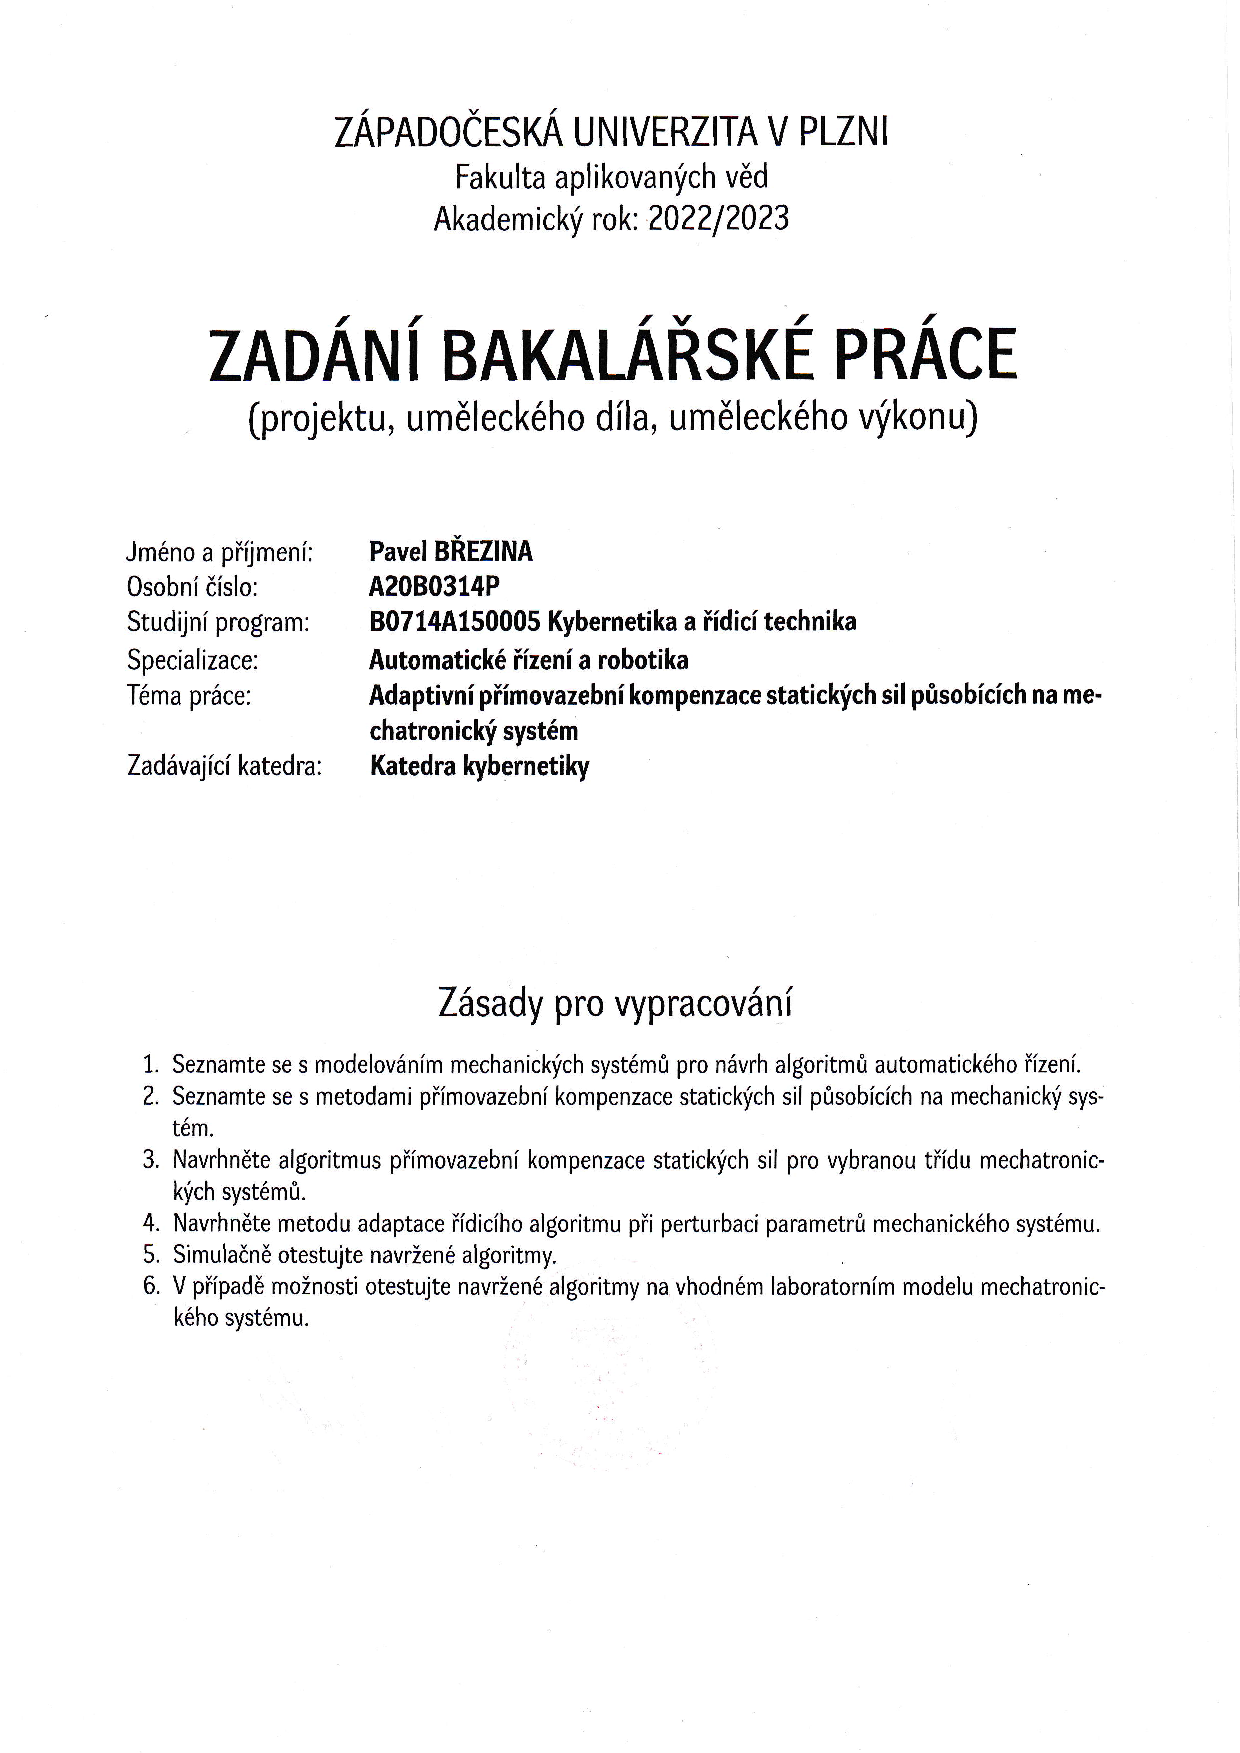
\includepdf[pages=-]{Img/Zadání BP.pdf}
\vspace*{\fill}
\section*{Prohlášení}
Předkládám tímto k posouzení a obhajobě bakalářskou práci zpracovanou
na závěr studia na Fakultě aplikovaných věd Západočeské univerzity v Plzni.
\par
Prohlašuji, že jsem bakalářskou práci vypracoval samostatně a výhradně s použitím odborné literatury
a pramenů, jejichž úplný seznam je její součástí.
\par
\vspace{5mm}
V Plzni dne \today \hfill ............................................
% \null\hfill Pavel Březina
\vspace*{\fill}
\newpage
\section*{Abstrakt}
Tato práce se zabývá automatickou kompenzací statických sil působících na mechatronický systém pomocí proudové kalibrační tabulky. Konkrétně se v práci prozkoumávají možnosti automatické aktualizace této tabulky pomocí NURBS interpolace a aproximace. Toto zahrnuje interpolaci a aproximaci 2D křivek, 3D křivek, 3D povrchů a 4D nadpovrchů, včetně jejich ukázek na obecných a konkrétních datech týkajících se problému této práce. Výsledkem práce je autonomní aktualizace proudové kalibrační tabulky za využití aproximace 4D nadpovrchu.
\section*{Klíčová slova}
\section*{Poděkování}
Rád bych poděkoval Ing. Václavu Helmovi, vedoucímu této bakalářské práce, za řádné vedení, přátelskou komunikaci a věnovaný čas pravidelným konzultacím, které značně pomohly směru vývoje této práce.
\newpage
